{\textbf{检错编码:}}就是通过一定的编码和解码,能够在接收端解码时检查出传输的错误,但不能纠正错误。常见的检错编码有奇偶校验码和循环冗余校验(CRC)码。

\textbf{1.奇偶校验码}

奇偶校验码就是在信息码后面加一位校验码,分为奇校验和偶校验。

\textbf{奇校验:}添加一位校验码后,使得整个码字里面1的个数是奇数;接收端收到数据后就校验数据里1的个数,如果正好为奇数,则认为传输没有出错;如果检测到偶数个1,则说明传输过程中,数据发生了改变,要求重发。

\textbf{偶校验:}添加一位校验码后,使得整个码字里面1的个数是偶数;接收端收到数据后就校验数据里1的个数,如果正好为偶数,则认为传输没有出错;如果检测到奇数个1,则说明传输过程中,数据发生了改变,要求重发。

\textbf{2.循环冗余校验(CRC)码}

奇偶校验码的检错率较低,不太实用。目前,在计算机网络和数据通信中,用得最广泛的就是检错率高、开销小、易实现的循环冗余校验码。循环冗余校验码的原理比较简单,相关教材讲解得很细致,这里不再赘述。以下仅给出考生在求解循环冗余校验码过程中遇到的一个最常见问题的解答,即循环冗余校验码中的二进制除法。

试计算10110010000/11001。

解析:解题技巧包括以下3个方面。

\textbf{1)}0±1=1,0±0=0,1±0=1,1±1=0(可以简化为做``异或''运算,在除法过程中,计算部分余数,全部使用``异或''操作,相同则为0,不同则为1)。

\textbf{2)}上商的规则是看部分余数的首位,如果为1,商上1;如果为0,商上0。

\textbf{3)}当部分余数的位数小于除数的位数时,该余数即为最后余数。

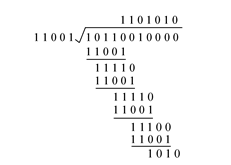
\includegraphics[width=2.40625in,height=1.71875in]{png-jpeg-pics/82DEB1BAC5D556F013E4B41211927DD0.png}

{\textbf{纠错编码:}}就是在接收端不但能检查出错误,而且能将检查出来的错误纠正。常见的纠错编码为\textbf{海明码}。

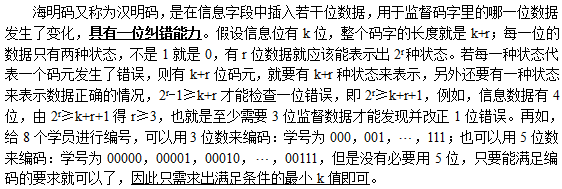
\includegraphics[width=3.69792in,height=1.23958in]{png-jpeg-pics/1871FE8447BD32C51FF14CE58A2608EA.png}
